% YOLO final 第一版阶段总结报告。
% 本报告只总结已经完成并具有正式记录的实验。
\documentclass[11pt,a4paper]{article}

\usepackage{CJKutf8}
\usepackage[a4paper,margin=1in]{geometry}
\usepackage{graphicx}
\usepackage{booktabs}
\usepackage{longtable}
\usepackage{float}
\usepackage{hyperref}
\usepackage{array}
\usepackage{caption}
\usepackage{amsmath}
\usepackage{amssymb}
\usepackage{multirow}
\usepackage{enumitem}
\pdfmapfile{+gbsnu.map}

\title{YOLO Final 阶段总结报告（Version 01）\\COCO-only 双尺度三框实验、DDP 训练链路与正式评估记录}
\author{}
\date{2026-05-03}

\begin{document}
\begin{CJK*}{UTF8}{gbsn}

\maketitle
\tableofcontents
\newpage

\section{实验目标与本报告覆盖范围}

本报告总结 \texttt{yolo\_final} 当前阶段已经完成的正式工作。报告的目的不是记录临时 smoke test，也不是提前讨论尚未完成的训练，而是把已经完成的 full-run、正式 COCO 评估、诊断修复和实验路线整理成一份可复现的阶段汇报。

截至本报告写作时，已经完成的主要内容包括：

\begin{enumerate}[label=\arabic*.]
  \item 修复 COCO 官方风格评估中的坐标空间错误；
  \item 将正式训练与评估口径从混合 VOC+COCO 调整为 COCO-only；
  \item 将数据读取补充为真正的 \texttt{.pt} packed loader，并在启动时校验数据口径；
  \item 将长训练从 \texttt{DataParallel} 改为 8GPU DDP；
  \item 完成 \texttt{lambda\_noobj=1.0}、\texttt{dynamic\_topk=1}、416 分辨率、K6 anchor、P3/K9 与 scale-aware routing 等正式实验；
  \item 对 K6 best checkpoint 完成非训练推理参数 sweep；
  \item 建立正式实验记录规范，包括配置、run id、checkpoint、COCO eval、diagnostics、可视化和 summary。
\end{enumerate}

本报告严格只记录已经完成并有正式结果的实验。未完成 full training、未完成 COCO 评估或只完成 smoke test 的实验不进入本报告结论。

\section{工程组织、数据来源与统一训练协议}

\subsection{工程目录}

本阶段全部工作位于 \texttt{/home/lidz/YOLO/yolo\_final}。关键目录包括：

\begin{itemize}
  \item \texttt{configs/}：正式训练配置；
  \item \texttt{models/}：Backbone、Neck、Head 与 Detector；
  \item \texttt{data/}：数据集读取与 target 组织；
  \item \texttt{losses/}：YOLO loss、动态匹配与多尺度监督；
  \item \texttt{engine/}：单机训练与 DDP 训练循环；
  \item \texttt{tools/}：训练、COCO 评估、checkpoint 诊断、推理 sweep 和图表导出；
  \item \texttt{logs/records/}：每次正式实验的配置快照、metadata 与结果文本；
  \item \texttt{outputs/}：checkpoint、评估结果、诊断可视化和报告图表；
  \item \texttt{runs/}：TensorBoard 事件文件；
  \item \texttt{report/}：诊断报告和阶段汇报。
\end{itemize}

\subsection{数据集与输入预处理}

当前正式实验使用 COCO-only 口径：

\begin{itemize}
  \item 训练集：\texttt{/home/lidz/YOLO/DataSet/Unified/manifests/coco2017\_train.jsonl}
  \item 验证集：\texttt{/home/lidz/YOLO/DataSet/Unified/manifests/coco2017\_val.jsonl}
  \item packed root：\texttt{/home/lidz/YOLO/DataSet/Unified/packed}
\end{itemize}

启动时会检查 packed dataset：train 为 118287 张 COCO train 图像，val 为 5000 张 COCO val 图像，类别空间为 COCO 80 类。

切换到 COCO-only 的原因是早期混合 \texttt{all\_train/all\_val} 直接拼接 VOC 与 COCO，但二者类别 id 语义不同。例如 label id 0 在 VOC 中是 aeroplane，在 COCO 中是 person。继续混合会让同一个分类输出接受冲突监督，因此正式结论统一使用 COCO-only。

\subsection{统一训练协议}

\begin{table}[H]
  \centering
  \caption{当前正式实验的主训练协议}
  \label{tab:shared-protocol}
  \begin{tabular}{ll}
    \toprule
    项目 & 当前设置 \\
    \midrule
    训练数据 & COCO-only \texttt{.pt} \\
    验证数据 & COCO val2017 \texttt{.pt} \\
    类别数 & 80 \\
    主输入尺寸 & 416 x 416 \\
    主特征层 & p4,p5 \\
    每尺度 anchor 数 & 3 \\
    训练轮数 & 30 \\
    优化器 & AdamW \\
    学习率调度 & cosine \\
    背景权重 & \texttt{lambda\_noobj=1.0} \\
    动态匹配 & \texttt{dynamic\_cost} \\
    正样本 top-k & \texttt{dynamic\_topk=2} \\
    多卡方式 & 8GPU DDP \\
    launcher & \texttt{torchrun --standalone --nproc\_per\_node=8} \\
    实验类型 & full training only \\
    \bottomrule
  \end{tabular}
\end{table}

smoke test 只用于 shape、语法、loss sanity check 和启动前校验，不进入正式结果表，也不作为实验结论。

\section{关键诊断与修复}

\subsection{COCO 评估坐标空间错误}

最初 COCO 评估结果异常接近 0。排查后确认预测框由模型在 resize 后坐标系中解码，而 COCO GT 使用原图坐标。旧评估直接把 resize 后坐标写入 COCO result，导致预测框与 GT 不在同一坐标空间。

\begin{table}[H]
  \centering
  \caption{COCO 坐标修复前后的官方风格指标}
  \label{tab:coco-coord-fix}
  \begin{tabular}{lrr}
    \toprule
    指标 & 修复前 & 修复后 \\
    \midrule
    COCO AP & 0.000240 & 0.121699 \\
    COCO AP50 & 0.000965 & 0.210424 \\
    COCO AP75 & 0.000016 & 0.122554 \\
    COCO AR@100 & 0.003765 & 0.263924 \\
    \bottomrule
  \end{tabular}
\end{table}

修复方式是在 \texttt{utils/coco\_eval.py} 中读取 \texttt{original\_size}，将预测框从 resize 坐标映射回原图宽高，并进行边界裁剪。修复后用 GT-as-pred oracle 验证，COCO AP/AP50 达到 1.0，说明评估链路正确。

\subsection{正样本统计维度错误}

旧版 \texttt{positive\_cells\_per\_image} 在多 anchor 情况下只对 H/W 求和，然后把 anchor 维也平均掉，导致日志中的正样本数被低估。该问题不影响训练梯度，但会影响我们判断 assignment 是否正常。修复后按每张图所有 grid 与 anchor 展平统计。

\subsection{\texttt{quality\_bce} 语义显式化}

配置中使用 \texttt{cls\_loss\_mode=quality\_bce} 与 \texttt{soft\_classification\_target=iou}。旧代码没有显式分支，容易造成配置语义不清。当前已将 \texttt{quality\_bce}、\texttt{bce}、\texttt{varifocal} 明确区分，并对未知模式报错。

\subsection{DDP 训练与日志语义}

早期 COCO-only 320 实验使用 \texttt{DataParallel}，20 epoch 训练和验证合计约 19.11 小时。补充 DDP 后，416 分辨率 30 epoch 训练约 6.9 小时，说明正式 8GPU DDP 是必要的。

DDP trainer 还补充了更严谨的日志语义：\texttt{steps} 表示 optimizer step，\texttt{global\_batches} 表示所有 rank 的 local batch 总数，epoch loss 按 sample count 加权，正式 COCO AP 通过独立评估脚本计算。

\section{第一阶段：COCO-only 与背景抑制}

第一阶段从修复后的混合数据实验转向 COCO-only，同时将 \texttt{lambda\_noobj} 提高到 1.0，以缓解候选框过多和误检重的问题。

\begin{table}[H]
  \centering
  \caption{COCO-only 320 \texttt{lambda\_noobj=1.0} 正式结果}
  \label{tab:coco-only-320}
  \begin{tabular}{ll}
    \toprule
    项目 & 数值 \\
    \midrule
    Run ID & \texttt{dual\_scale\_three\_box\_coco\_only\_noobj1\_20260428\_180817} \\
    Config & \texttt{configs/dual\_scale\_three\_box\_coco\_only\_noobj1.toml} \\
    多卡方式 & DataParallel \\
    输入尺寸 & 320 \\
    最优 epoch & 20 \\
    最优验证损失 & 5.262634 \\
    COCO AP / AP50 / AP75 & 0.126985 / 0.218369 / 0.129184 \\
    COCO AR100 & 0.260567 \\
    预测框/图 & 41.36 \\
    \bottomrule
  \end{tabular}
\end{table}

该实验相比修复后的混合数据 run，AP/AP50/AP75 小幅提升，AR100 略降。这符合增强背景抑制后的预期：排序和精度略好，但召回略受影响。该实验同时暴露出 \texttt{DataParallel} 训练太慢，因此下一步转向 DDP。

\section{第二阶段：DDP 与 \texttt{dynamic\_topk=1} 对照}

由于双尺度 p4/p5 会分别进行动态匹配，\texttt{dynamic\_topk=2} 可能让每个 GT 在多个尺度上产生较多正样本。该阶段测试 \texttt{dynamic\_topk=1} 是否能降低候选密度并改善官方指标。

\begin{table}[H]
  \centering
  \caption{\texttt{dynamic\_topk=1} 对照实验}
  \label{tab:topk1}
  \begin{tabular}{ll}
    \toprule
    项目 & 数值 \\
    \midrule
    Run ID & \texttt{dual\_scale\_three\_box\_coco\_only\_noobj1\_topk1\_ddp\_20260429\_144209} \\
    Config & \texttt{configs/dual\_scale\_three\_box\_coco\_only\_noobj1\_topk1.toml} \\
    多卡方式 & 8GPU DDP \\
    输入尺寸 & 320 \\
    最优 epoch & 20 \\
    最优验证损失 & 5.148357 \\
    验证 pos cells/image & 14.097600 \\
    COCO AP / AP50 / AP75 & 0.108180 / 0.195980 / 0.105638 \\
    COCO AR100 & 0.239071 \\
    \bottomrule
  \end{tabular}
\end{table}

\texttt{dynamic\_topk=1} 确实降低了正样本数，并让 validation loss 降低。但 COCO AP 和 AR100 都明显下降。因此，top-k 降低不是当前主线，\texttt{dynamic\_topk=2} 对召回和 ranking 更有价值。

\section{第三阶段：提升输入分辨率到 416}

在确认 DDP 训练链路可用后，下一步测试分辨率提升是否能直接改善检测质量。该阶段将输入从 320 提升到 416，保持 COCO-only、\texttt{lambda\_noobj=1.0} 与 \texttt{dynamic\_topk=2}。

\begin{table}[H]
  \centering
  \caption{416 分辨率原 anchor baseline}
  \label{tab:416-baseline}
  \begin{tabular}{ll}
    \toprule
    项目 & 数值 \\
    \midrule
    Run ID & \texttt{dual\_scale\_three\_box\_coco\_only\_noobj1\_416\_ddp\_20260430\_124818} \\
    Config & \texttt{configs/dual\_scale\_three\_box\_coco\_only\_noobj1\_416.toml} \\
    输入尺寸 & 416 \\
    特征层 & p4,p5 \\
    最优 epoch / 最优验证损失 & 23 / 4.779924 \\
    COCO AP / AP50 / AP75 & 0.148786 / 0.248717 / 0.155263 \\
    AP small/medium/large & 0.056 / 0.159 / 0.214 \\
    COCO AR100 & 0.302299 \\
    预测框/图 & 52.05 \\
    \bottomrule
  \end{tabular}
\end{table}

\begin{table}[H]
  \centering
  \caption{320 到 416 的改进幅度}
  \label{tab:320-to-416}
  \begin{tabular}{lrrr}
    \toprule
    指标 & 320 topk2 & 416 topk2 & 变化 \\
    \midrule
    Best val loss & 5.262634 & 4.779924 & -0.482710 \\
    AP & 0.126985 & 0.148786 & +0.021801 \\
    AP50 & 0.218369 & 0.248717 & +0.030348 \\
    AP75 & 0.129184 & 0.155263 & +0.026079 \\
    AR100 & 0.260567 & 0.302299 & +0.041732 \\
    \bottomrule
  \end{tabular}
\end{table}

提高分辨率是当前最明确的正向改动。AP、AP50、AP75 和 AR100 同时提升。因此 416 原 anchor run 成为当前 AP baseline。

\section{第四阶段：COCO train GT box 重新聚类 K6 anchors}

在 416 baseline 上，使用 COCO train GT box 重新聚类得到 K6 anchors，并比较其是否能改善训练稳定性、召回和官方 COCO 指标。

\begin{table}[H]
  \centering
  \caption{416 K6 anchors 默认推理结果}
  \label{tab:k6-default}
  \begin{tabular}{ll}
    \toprule
    项目 & 数值 \\
    \midrule
    Run ID & \texttt{dual\_scale\_three\_box\_coco\_only\_noobj1\_416\_k6\_ddp\_20260501\_024802} \\
    Config & \texttt{configs/dual\_scale\_three\_box\_coco\_only\_noobj1\_416\_k6.toml} \\
    输入尺寸 & 416 \\
    特征层 & p4,p5 \\
    anchors & COCO train K6 \\
    最优 epoch / 最优验证损失 & 23 / 4.694147 \\
    COCO AP / AP50 / AP75 & 0.146778 / 0.244778 / 0.153023 \\
    AP small/medium/large & 0.059 / 0.156 / 0.210 \\
    COCO AR100 & 0.303445 \\
    预测框/图 & 51.92 \\
    \bottomrule
  \end{tabular}
\end{table}

默认推理下，K6 降低了 best val loss，并略微提高 AR100，但 AP/AP50/AP75 略低于 416 原 anchor baseline。

\subsection{K6 best checkpoint 非训练 sweep}

K6 best checkpoint 完成了非训练推理参数 sweep。先在 500 张 COCO val 上进行 broad sweep，再对候选设置跑完整 COCO val。

\begin{table}[H]
  \centering
  \caption{K6 best checkpoint 完整 COCO 推理 sweep}
  \label{tab:k6-sweep}
  \begin{tabular}{lrrrrr}
    \toprule
    推理设置 & AP & AP50 & AP75 & AP small & AR100 \\
    \midrule
    default & 0.146778 & 0.244778 & 0.153023 & 0.059000 & 0.303445 \\
    AP-best & 0.147754 & 0.247426 & 0.153436 & 0.060051 & 0.323725 \\
    AP50-best & 0.146959 & 0.248385 & 0.152309 & 0.058978 & 0.311373 \\
    AR-best & 0.146512 & 0.239456 & 0.155499 & 0.060166 & 0.335957 \\
    \bottomrule
  \end{tabular}
\end{table}

推荐的平衡推理配置为 \texttt{score\_alpha=2.0}、\texttt{score\_beta=1.0}、\texttt{score\_threshold=0.01}、\texttt{top\_k=200}、\texttt{nms\_iou\_threshold=0.5}。

K6 不是默认 AP 最强点，但它在 tuned inference 下几乎追平 416 原 anchor AP baseline，并显著提高 AR100。因此 K6 是当前最值得继续做训练侧改进的路线。

\section{第五阶段：增加 P3 与 K9 anchors}

在 416 基础上增加 P3，形成 p3/p4/p5 三尺度输出，并使用 COCO train K9 anchors。该实验的核心问题是：P3 是否能改善小目标和召回。

\begin{table}[H]
  \centering
  \caption{416 P3/P4/P5 K9 all-scale 实验结果}
  \label{tab:p3-k9}
  \begin{tabular}{ll}
    \toprule
    项目 & 数值 \\
    \midrule
    Run ID & \texttt{dual\_scale\_three\_box\_coco\_only\_noobj1\_416\_p3p4p5\_k9\_ddp\_20260501\_140417} \\
    Config & \texttt{configs/dual\_scale\_three\_box\_coco\_only\_noobj1\_416\_p3p4p5\_k9.toml} \\
    特征层 / anchors & p3,p4,p5 / COCO train K9 \\
    参数量 / GFLOPs & 41,451,613 / 100.309747 \\
    最优 epoch / 最优验证损失 & 19 / 6.605443 \\
    COCO AP / AP50 / AP75 & 0.136481 / 0.228555 / 0.143862 \\
    AP small / AR small & 0.062 / 0.125 \\
    COCO AR100 & 0.313965 \\
    \bottomrule
  \end{tabular}
\end{table}

P3/K9 提高了 AP small 和 AR100，但总 AP、AP50、AP75 下降。这说明 P3 提供了有用候选召回，但当前 all-scale matching 增加了 ranking 和 NMS 压力。

\section{第六阶段：严格 scale-aware routing}

上一阶段 P3 提高了召回但降低 AP。为了减少同一个 GT 在多个尺度上的重复监督，下一步加入严格面积路由：\texttt{scale\_assignment=area}，\texttt{scale\_area\_thresholds=0.18,0.35}。

\begin{table}[H]
  \centering
  \caption{P3/P4/P5 K9 scale-aware routing 结果}
  \label{tab:p3-area}
  \begin{tabular}{ll}
    \toprule
    项目 & 数值 \\
    \midrule
    Run ID & \texttt{dual\_scale\_three\_box\_coco\_only\_noobj1\_416\_p3p4p5\_k9\_scaleaware\_ddp\_20260502\_141852} \\
    Config & \texttt{configs/dual\_scale\_three\_box\_coco\_only\_noobj1\_416\_p3p4p5\_k9\_scaleaware.toml} \\
    scale assignment / thresholds & area / 0.18, 0.35 \\
    最优 epoch / 最优验证损失 & 21 / 4.485392 \\
    验证 pos cells/image & 14.600800 \\
    COCO AP / AP50 / AP75 & 0.120353 / 0.198501 / 0.124782 \\
    AP small / AR100 & 0.052 / 0.298278 \\
    \bottomrule
  \end{tabular}
\end{table}

严格面积路由把 pos cells/image 从约 42.94 降到 14.60，也把 best val loss 从 6.605443 降到 4.485392。但 COCO AP 从 0.136481 降到 0.120353。这说明 validation loss 的下降主要来自正样本减少和重复监督减少，并不等价于检测质量提升。

因此，严格独占 \texttt{scale\_assignment=area} 被拒绝作为下一版 baseline。如果后续继续 P3，应使用更软的控制方式，例如 P3 loss/objectness down-weight 或 overlapping area assignment。

\section{正式实验综合对比}

\begin{figure}[H]
  \centering
  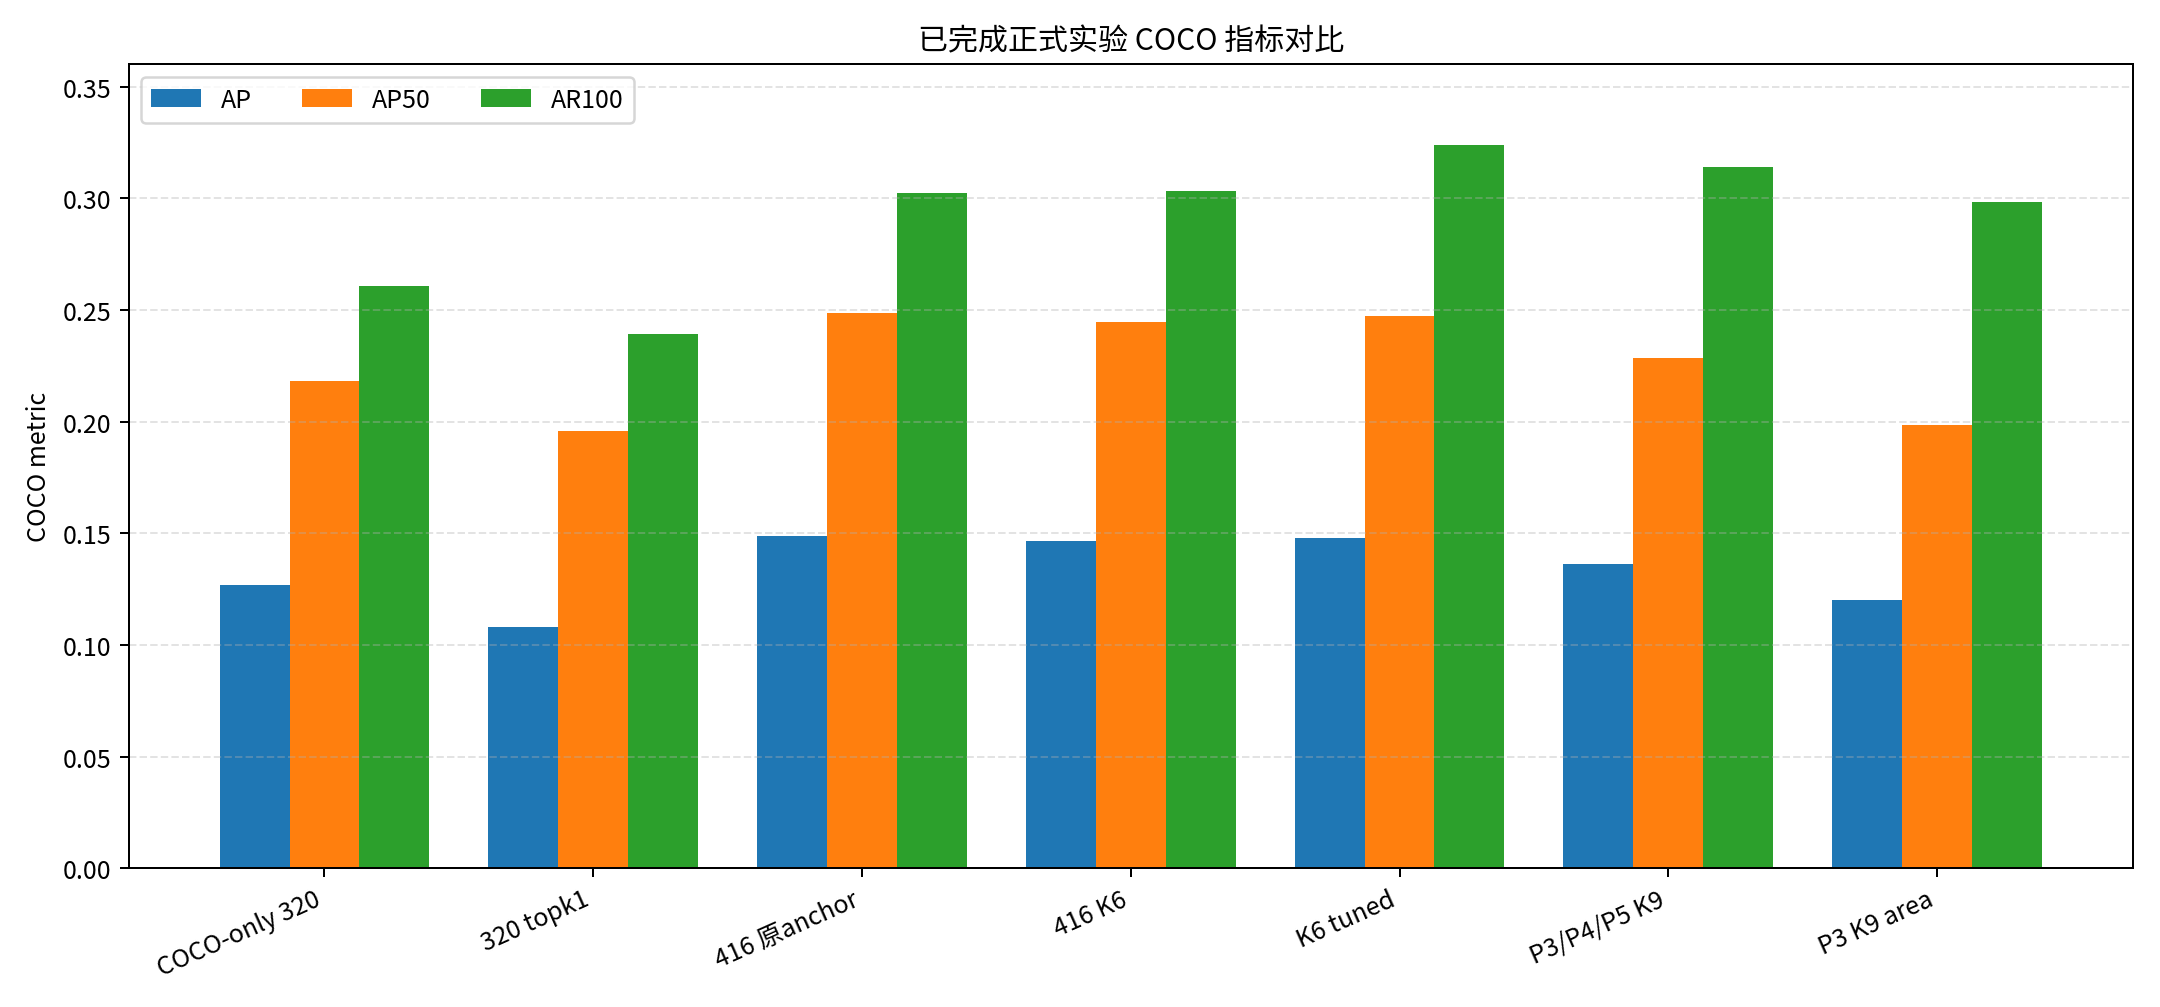
\includegraphics[width=0.98\textwidth]{../outputs/report_assets/final_version1/completed_coco_metrics.png}
  \caption{已完成正式实验的 COCO AP、AP50 与 AR100 对比。}
  \label{fig:coco-metrics}
\end{figure}

\begin{figure}[H]
  \centering
  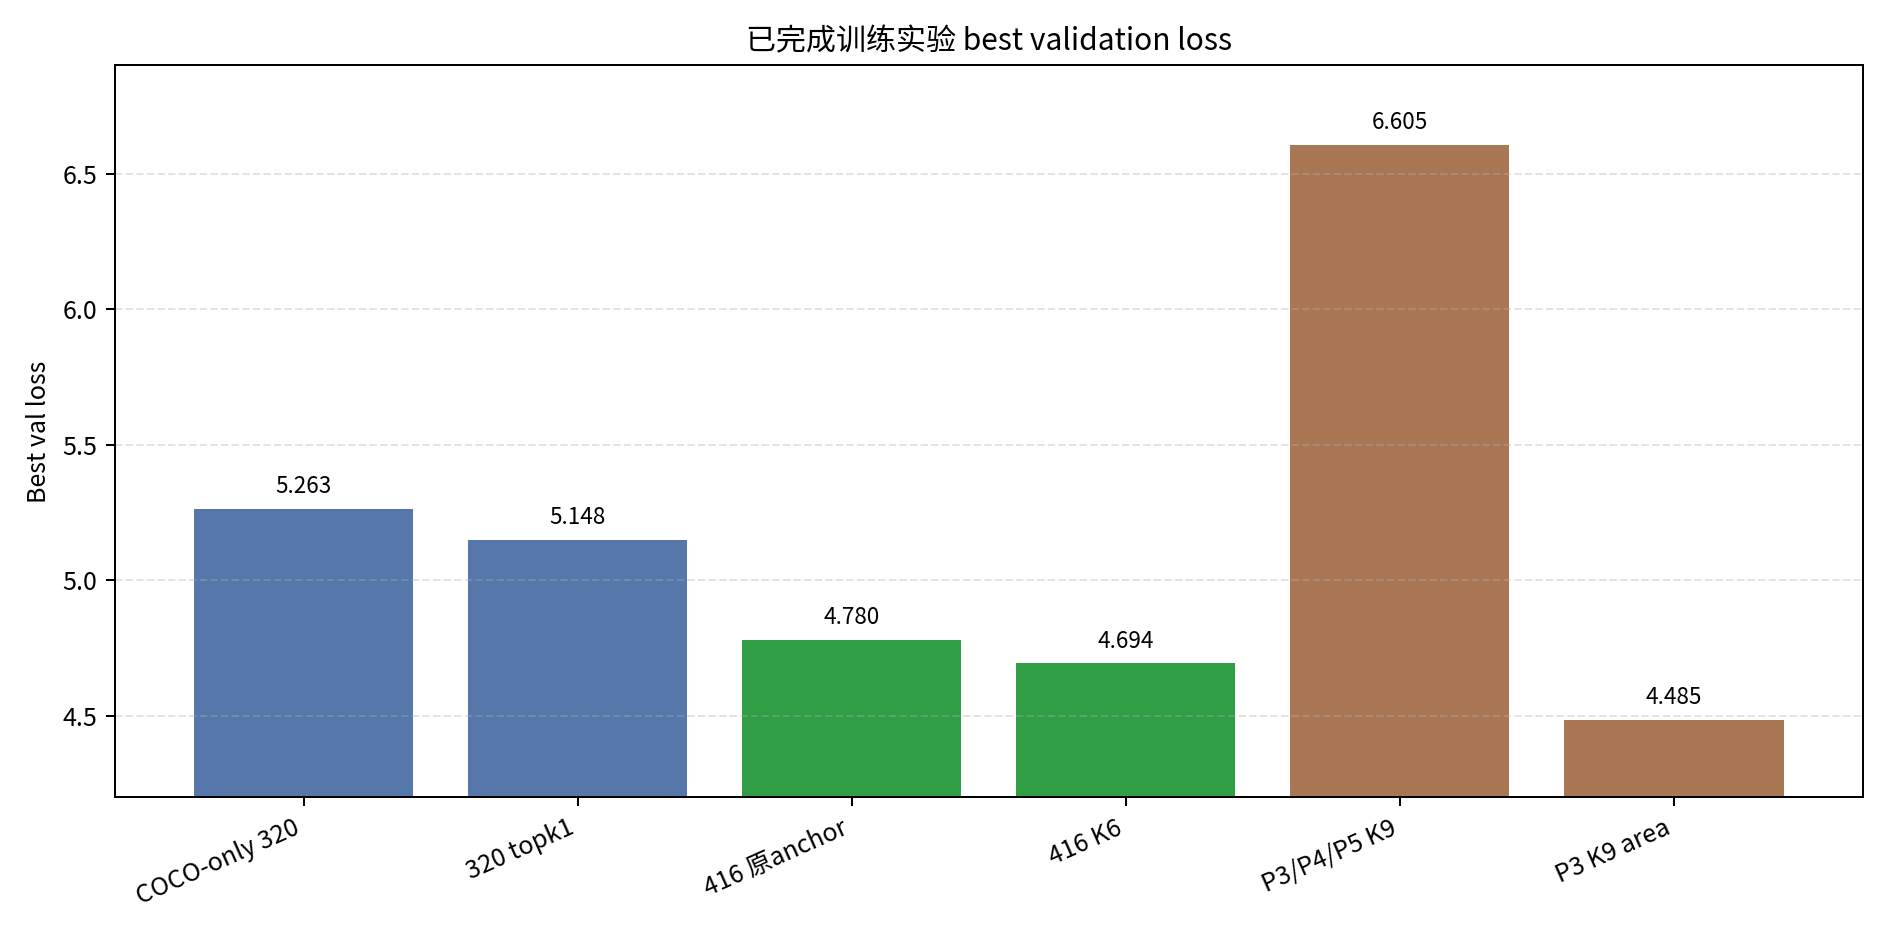
\includegraphics[width=0.92\textwidth]{../outputs/report_assets/final_version1/completed_val_loss.png}
  \caption{已完成训练实验的 best validation loss 对比。K6 tuned inference 是非训练 sweep，因此不纳入该图。}
  \label{fig:val-loss}
\end{figure}

\begin{figure}[H]
  \centering
  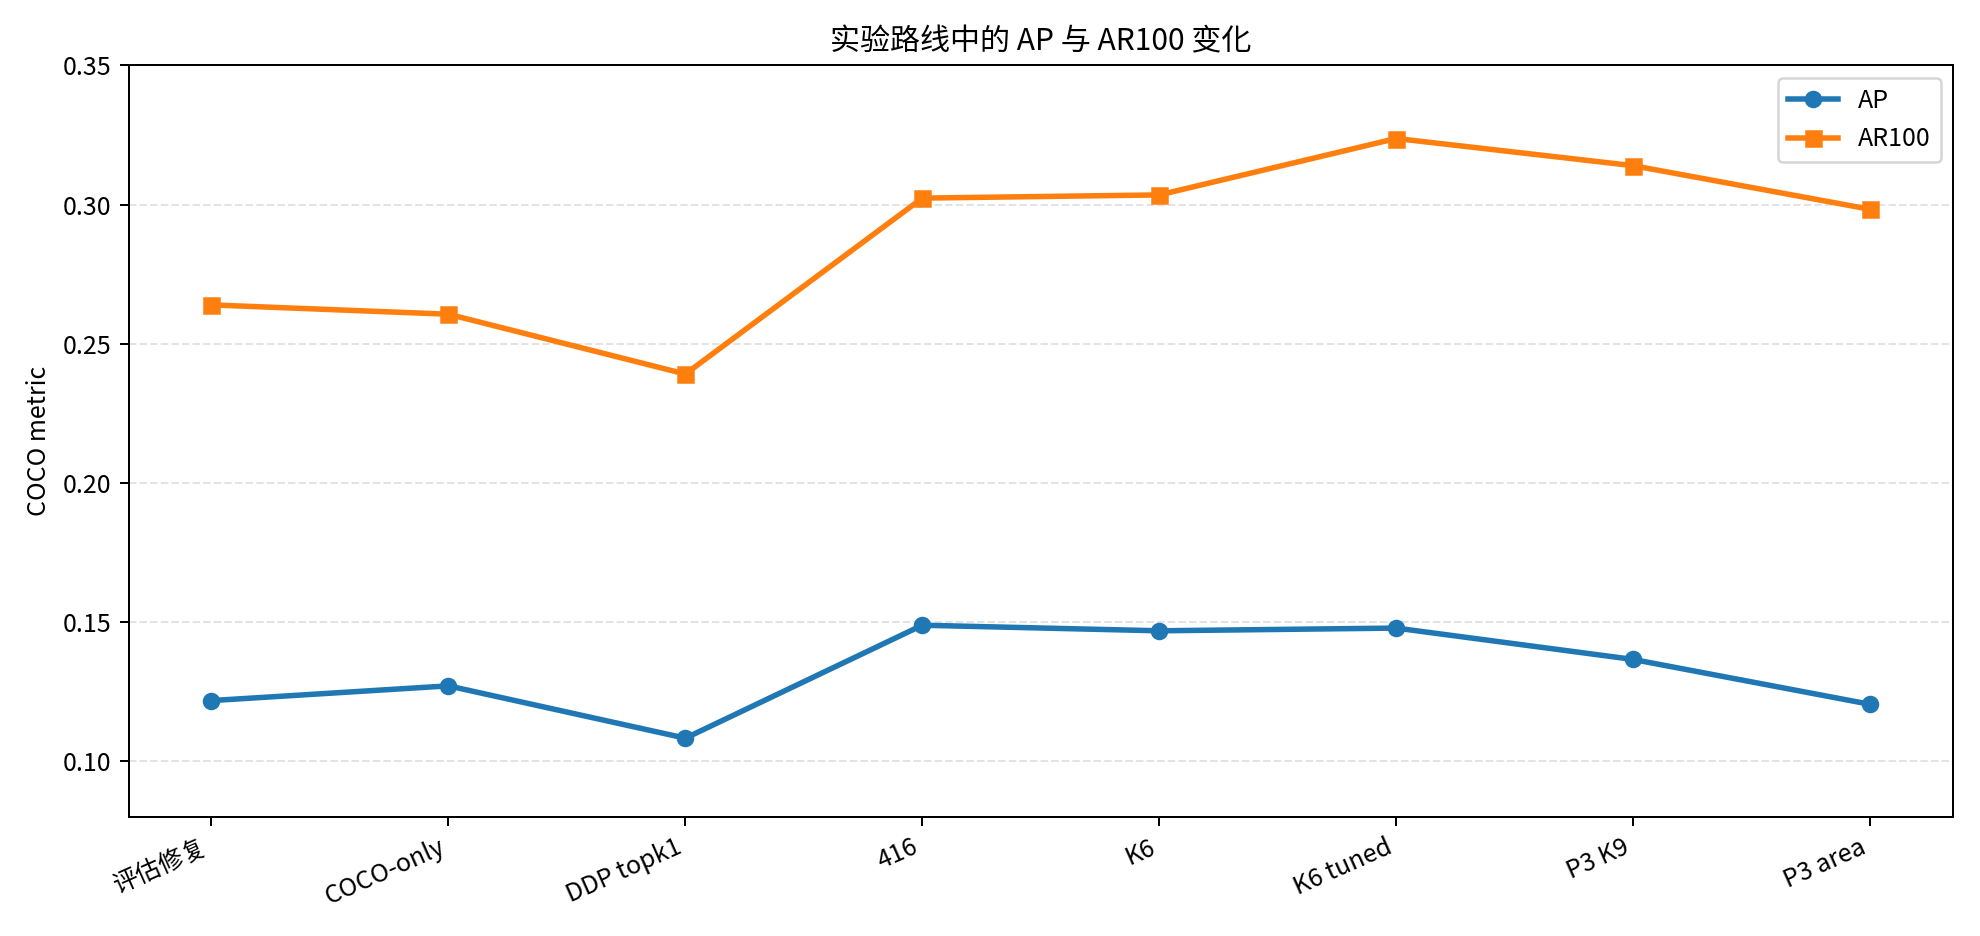
\includegraphics[width=0.96\textwidth]{../outputs/report_assets/final_version1/route_ap_ar100.png}
  \caption{实验路线中的 AP 与 AR100 变化。}
  \label{fig:route-ap-ar}
\end{figure}

\begin{longtable}{lrrrrl}
  \caption{已完成正式实验主指标汇总}
  \label{tab:all-results}\\
  \toprule
  实验 & AP & AP50 & AP75 & AR100 & 结论 \\
  \midrule
  \endfirsthead
  \toprule
  实验 & AP & AP50 & AP75 & AR100 & 结论 \\
  \midrule
  \endhead
  修复评估后的混合数据 run & 0.121699 & 0.210424 & 0.122554 & 0.263924 & 工程验证 \\
  COCO-only 320 topk2 & 0.126985 & 0.218369 & 0.129184 & 0.260567 & COCO-only 起点 \\
  COCO-only 320 topk1 & 0.108180 & 0.195980 & 0.105638 & 0.239071 & 负向结果 \\
  COCO-only 416 原 anchor & 0.148786 & 0.248717 & 0.155263 & 0.302299 & 当前 AP baseline \\
  COCO-only 416 K6 & 0.146778 & 0.244778 & 0.153023 & 0.303445 & val loss 更低 \\
  K6 tuned inference & 0.147754 & 0.247426 & 0.153436 & 0.323725 & 实用召回 baseline \\
  P3/P4/P5 K9 & 0.136481 & 0.228555 & 0.143862 & 0.313965 & 小目标和召回信号 \\
  P3/P4/P5 K9 area & 0.120353 & 0.198501 & 0.124782 & 0.298278 & 严格路由失败 \\
  \bottomrule
\end{longtable}

\section{当前最优判断}

从已经完成的实验看，当前结论如下：

\begin{itemize}
  \item 当前 AP baseline 是 \texttt{dual\_scale\_three\_box\_coco\_only\_noobj1\_416\_ddp\_20260430\_124818}，AP 为 0.148786。
  \item 当前实用召回 baseline 是 416 K6 + tuned inference，AP 为 0.147754，AR100 为 0.323725。
  \item \texttt{dynamic\_topk=1} 不应作为主线，因为它降低了 AP 和 AR。
  \item P3/K9 有小目标和召回价值，但当前版本不能替代 416 p4/p5 baseline。
  \item 严格 area routing 不能用 validation loss 作为成功依据，COCO AP/AR 是最终判断标准。
  \item 候选框密度仍然偏高，diagnostics 多次显示 top-k 饱和，这是下一阶段需要继续解决的问题。
\end{itemize}

\section{优良实验记录规范}

\subsection{正式实验准入}

后续只有满足以下条件的实验才进入正式对比表：

\begin{enumerate}[label=\arabic*.]
  \item 使用固定配置文件启动；
  \item 通过 smoke/sanity check；
  \item 完成 full training；
  \item 保存 best/last checkpoint；
  \item 完成完整 COCO val2017 评估；
  \item 完成 checkpoint diagnostics；
  \item 写入 summary 和 \texttt{experiment\_result\_index.md}；
  \item 对关键指标给出明确结论。
\end{enumerate}

smoke test、失败启动、未完成训练、未完成正式 COCO 评估的 run 只作为排查记录，不进入正式结果表。

\subsection{每次实验必须保存的内容}

每次正式实验至少保存配置文件路径、配置快照、run id、tmux session、训练日志、output dir、best checkpoint、last checkpoint、TensorBoard 目录、COCO eval JSON、diagnostics JSON、diagnostic visualizations、summary markdown、metadata JSON，并在 \texttt{logs/experiment\_result\_index.md} 中登记。

\subsection{必须记录的指标}

训练指标包括 total/box/objectness/classification loss、GIoU、pos cells/image、dropped GT/image、ignored candidates/image、optimizer steps、global batches、train/val loop time、GPU 占用和 8GPU DDP 进程状态。

评估指标包括 COCO AP@[.50:.95]、AP50、AP75、AP small/medium/large、AR1、AR10、AR100、AR small/medium/large、predictions 总数、predictions/image、score quantiles，以及 score threshold、top-k、NMS sweep 结果。

\section{下一步方向}

下一步应围绕已经证明最有价值的 416/K6 路线继续改进，而不是马上回到 P3。

优先级建议如下：

\begin{enumerate}[label=\arabic*.]
  \item 保持 416、p4/p5、K6、\texttt{lambda\_noobj=1.0}、\texttt{dynamic\_topk=2}；
  \item 优先研究训练侧 assignment 与 score calibration；
  \item 对所有新训练使用同一 tuned inference 口径评估；
  \item 如果 K6 路线无法继续提高 AP，再回到 P3，但采用软控制而不是严格独占 routing；
  \item 每次训练只改一个主要变量，避免同时改变分辨率、anchor、尺度和 loss。
\end{enumerate}

后续可选方向包括 anchor shape prior cost sweep、objectness target 质量加权、Varifocal/QFL 方向的分类质量建模、P3 all-scale + P3 loss/objectness 下调，以及 overlapping area assignment。

\section{总结}

当前阶段已经完成从“能训练”到“能可信比较”的转变。最关键的工程成果包括 COCO 评估坐标修复、COCO-only 数据口径、\texttt{.pt} loader、8GPU DDP、loss 统计修复、正式 COCO eval、checkpoint diagnostics 和实验记录索引。

从实验结果看，416 分辨率是最确定的正向改动；K6 anchors 在默认推理下 AP 略低，但通过非训练 sweep 后几乎追平 AP baseline，并明显提高 AR100；P3/K9 证明了小目标和召回潜力，但当前版本的候选密度和排序压力仍然过大；严格 scale-aware routing 说明 validation loss 不能替代 COCO AP/AR。

因此，当前最稳妥的结论是：以 416 原 anchor 作为 AP baseline，以 416 K6 tuned inference 作为实用召回 baseline，后续训练改进优先围绕 K6 的 assignment 与 score calibration 展开。

\appendix

\section{关键记录路径}

\begin{itemize}
  \item 实验索引：\texttt{logs/experiment\_result\_index.md}
  \item 诊断报告：\texttt{report/诊断.tex}
  \item K6 sweep 记录：\texttt{logs/k6\_best\_checkpoint\_nontraining\_sweep\_20260502.md}
  \item 图表输出：\texttt{outputs/report\_assets/final\_version1/}
  \item COCO 评估脚本：\texttt{tools/evaluate\_coco.py}
  \item checkpoint 诊断脚本：\texttt{tools/diagnose\_coco\_checkpoint.py}
  \item 非训练 sweep 脚本：\texttt{tools/sweep\_coco\_checkpoint.py}
\end{itemize}

\end{CJK*}
\end{document}
